\noindent\begin{minipage}{7cm}
\begin{description}
\item[Objectif :] imbriquer des boucles.
\item[Syntaxe \python :] \mbox{}
\begin{itemize}
\item \texttt{for element in sequence : \\ \mbox{}\ \ \ \ blocFor}

\item \texttt{range([start,] end [, step])}\\ crée une liste d'entiers compris 
entre \texttt{\tt start} inclus
($= 0$ par défaut) et \texttt{end} exclus par pas de \texttt{step} ($= 1$ par défaut).
\end{itemize}
\end{description}
\end{minipage}
\mbox{}\hfill
\begin{tabular}{c}
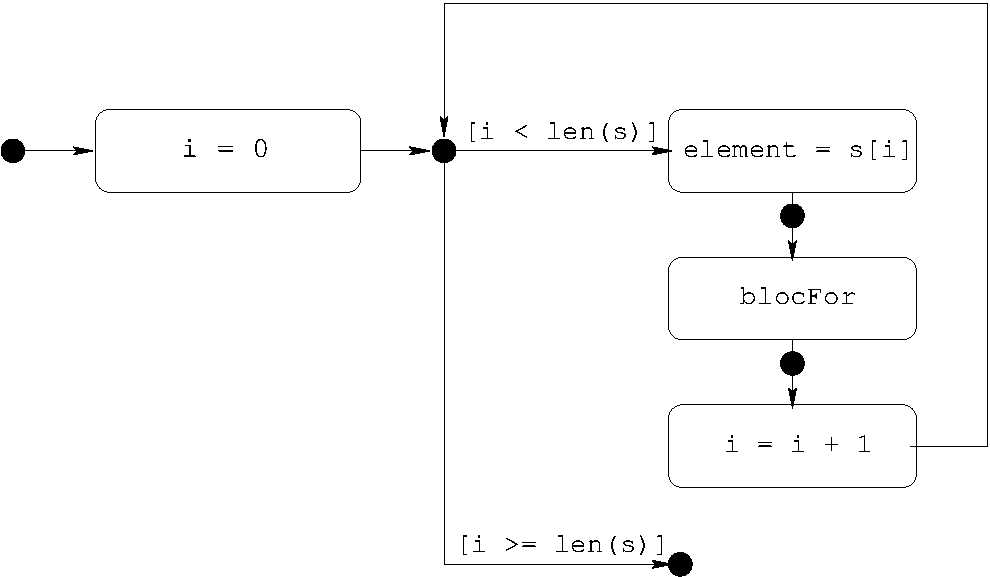
\includegraphics[width=7.5cm]{uml7.pdf}\\
\end{tabular}

%-------------------------------------------------------------------------
\subsection{Exemple}
%-------------------------------------------------------------------------

\paragraph{Enoncé} On dispose d'un tas de bois formé de rondins d'environ $1 m$ de long et
de $10 cm$ de diamètre, et on veut les liter en quinconce régulier pour former un stère 
de bois ($1m\times 1m\times 1m = 1 m^3$). 

\noindent\begin{minipage}{9cm}
On suppose que des pieux verticaux sont disposés aux quatre coins du stère pour éviter la chute des rondins périphériques.
\end{minipage}
\hfill
\begin{minipage}{3cm}
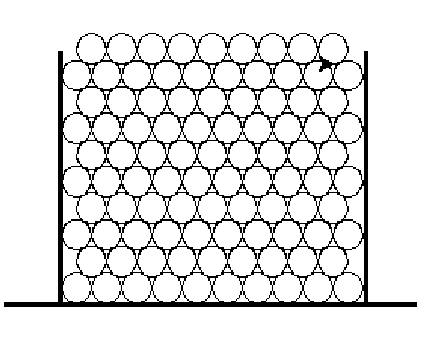
\includegraphics[width=3cm]{stere.pdf}
\end{minipage}

\paragraph{Méthode} On commence par poser sur le sol une première couche horizontale
de 10 rondins; on dispose par dessus en quinconce une deuxième rangée de 9 rondins puis
une troisième rangée de 10 rondins, et ainsi de suite jusqu'à superposer
$10$ rangées horizontales alternativement de 10 et 9 rondins.

\paragraph{Questions} 
On décompose le problème en deux sous-problèmes : empiler des rangées, aligner des rondins pour faire une rangée.

\begin{question}[«~ranger le bois~» : les rangées] Proposer un algorithme pour 
construire un stère de bois en supposant que l'on sait manipuler directement
une rangée horizontale de rondins.
\end{question}

\begin{question}[«~ranger le bois~» : une rangée] Proposer un algorithme
pour construire une rangée horizontale de rondins de bois.
\end{question}

\begin{question}[«~ranger le bois~» : le stère] Proposer un algorithme
pour construire un stère de \linebreak bois.
\end{question}


%-------------------------------------------------------------------------
\subsection{Généralisation}
%-------------------------------------------------------------------------
Une boucle permet de traiter une séquence d'éléments un par un, 
les uns après les autres (\emph{placer une rangée, puis une autre, puis une autre\ldots}), et pour chaque élément, 
on peut vouloir traiter autre chose de manière systématique (\emph{aligner les rondins}).
L'algorithme sera ainsi constitué d'une boucle principale (\emph{qui place les rangées}) et
dans le corps de cette boucle principale, on dit aussi «~à l'intérieur de la boucle~», 
une boucle secondaire (\emph{qui aligne les rondins pour faire une rangée}).
La boucle secondaire peut elle-même contenir une boucle, et ainsi de suite.


\begin{question}[boucles imbriquées : exécutions]
Qu'affichent les itérations suivantes ?

\begin{minipage}[t]{6cm}\tt
\begin{Verbatim}
for i in range(10) :
    j = 10 - i
    while j > 0 :
        print('*',end='')
        j = j - 1
    print()
\end{Verbatim}
\end{minipage}
\hfill
\begin{minipage}[t]{6cm}\tt
\begin{Verbatim}
i = 0
while i < 10 :
    for j in range(i) :
        print('*',end='')
    print()
    i = i + 1
\end{Verbatim}
\end{minipage}

\end{question}

L'approche efficace pour résoudre un problème (\emph{ranger le bois}) consiste
souvent à le décomposer en plusieurs sous-problèmes plus simples
(\emph{placer une rangée}\ldots) qui seront étudiés
séparément. Ces sous-problèmes peuvent éventuellement être eux-mêmes décomposés 
à leur tour (\emph{aligner les rondins}\ldots), et ainsi de suite.
Le concepteur de l'algorithme définit la structuration d'un problème en sous-problèmes : 
il divise le problème en sous-problèmes pour mieux le contrôler (\emph{diviser pour régner}).
Lorsque les problèmes et sous-problèmes correspondent à des boucles, on obtiendra
une structuration en boucles imbriquées et/ou en boucles successives.

\begin{question}[boucles imbriquées : imbriquées ou successives ?]
A partir de deux exemples sim\-ples et comparables, illustrer et expliquer la différence
entre deux boucles imbriquées et deux boucles successives.
Dessiner les diagrammes \uml{} correspondants.
\end{question}

%-------------------------------------------------------------------------
\subsection{Applications}
%-------------------------------------------------------------------------
\begin{question}[boucles imbriquées : tables de vérité] Ecrire un algorithme qui affiche
la table de vérité du circuit logique suivant, où $a$, $b$ et $c$ sont les entrées et 
$s_0, s_1, \ldots, s_7$ les sorties.
$$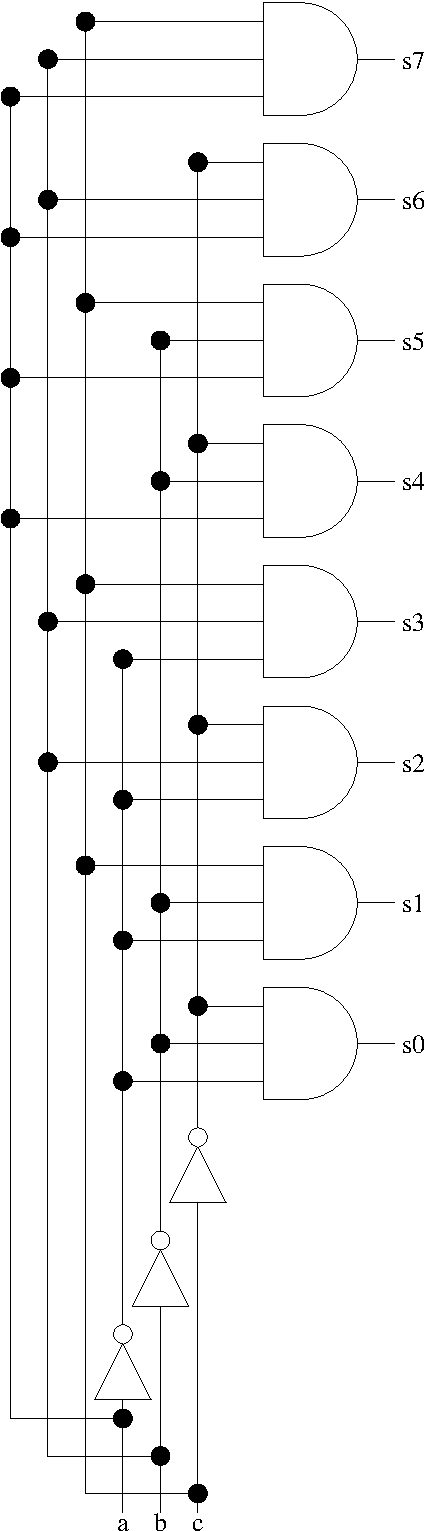
\includegraphics[width=4cm,angle=90]{decodeur.pdf}$$
\end{question}

\begin{question}[boucles imbriquées : tables de multiplication] Ecrire un algorithme
qui affiche\linebreak successivement les 10 premières tables de multiplication de deux manières 
différentes : \\
d'abord sous la forme :
\begin{minipage}[t]{3cm}\tt
\begin{Verbatim}
3 x 0 = 0
3 x 1 = 3
3 x 2 = 6
3 x 3 = 9
...
3 x 9 = 27
\end{Verbatim}
\end{minipage}
\hfill
puis sous la forme :
\begin{minipage}[t]{3cm}\tt
\begin{Verbatim}
0 x 3 = 0
1 x 3 = 3
2 x 3 = 6
3 x 3 = 9
...
9 x 3 = 27
\end{Verbatim}
\end{minipage}
\end{question}

\begin{question}[boucles imbriquées : triangle de Pascal] Ecrire un algorithme qui affiche le triangle de Pascal jusqu'à l'ordre $n$. 
Chaque ligne $i$ de ce triangle est composée des coefficients $c_{ij}$ du binôme 
$\displaystyle (x + y)^i = \sum_{j=0}^{i} c_{ij}x^{i-j}y^j = \sum_{j=0}^{i} \frac{i!}{j!(i-j)!}x^{i-j}y^j$ où $\forall i,$ $c_{i0} = c_{ii} = 1$ et $c_{ij} = c_{i-1,j} + c_{i-1,j-1}$ $\forall j,\ 0 < j < i$.

\noindent
Les 8 premières lignes du triangle de Pascal sont donc les suivantes :
\hfill\begin{minipage}[t]{4cm}\tt
\begin{Verbatim}
1
1 1
1 2 1
1 3 3 1
1 4 6 4 1
1 5 10 10 5 1
1 6 15 20 15 6 1
1 7 21 35 35 21 7 1
\end{Verbatim}
\end{minipage}	
\end{question}

%\begin{question}[boucles imbriquées : produits de matrices] Ecrire un algorithme qui calcule
%le produit $C$ de 2 matrices $A$ et $B$ respectivement de dimensions $(n,r)$ et $(r,m)$.
%
%$$\begin{minipage}{5cm}
%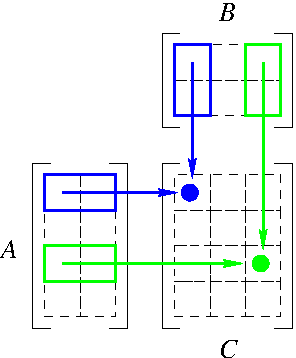
\includegraphics[width=4cm]{produit-matrices.pdf}
%\end{minipage}
%\hspace*{1cm}
%c_{ij} = \sum_{k=0}^{r-1}a_{ik}\cdot b_{kj}$$
%
%\end{question}


%-------------------------------------------------------------------------
%\newpage
\subsection{Entraînement}
%-------------------------------------------------------------------------

%-------------------------------------------------------------------------
\subsubsection{Enoncé}
%-------------------------------------------------------------------------

\paragraph{Objectif :} en utilisant les instructions de la tortue \logo{}
(module \texttt{turtle}), écrire un algorithme qui dessine un motif géométrique
régulier composé de polygones réguliers.


\paragraph{Méthode :} 
construire l'algorithme en décomposant le problème en 3 niveaux :
\begin{enumerate}
\item le tracé du polygone élémentaire,
\item le tracé d'une ligne de polygones élémentaires,
\item le tracé du motif de lignes de polygones élémentaires.
\end{enumerate}
On pourra commencer soit par l'étape de plus haut niveau (le motif), 
soit par l'étape de plus bas niveau (le polygone élémentaire).

\paragraph{Vérification :} vérifier l'algorithme sous \python{} en comparant 
le tracé obtenu avec la figure de l'énoncé.

%-------------------------------------------------------------------------
\subsubsection{Exemple}
%-------------------------------------------------------------------------
On considère le motif composé de ($5\times 4$)
hexagones réguliers de côté de longueur $d$ représenté ci-dessous :

$$\begin{minipage}{6.75cm}
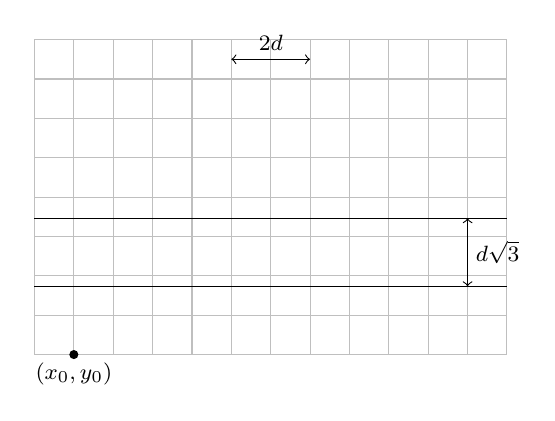
\begin{tikzpicture}[scale=0.5]\footnotesize
\draw[color=lightgray](-6,-4) grid[xstep=1,ystep=1] (6,4);
%\foreach \x in {-6,-5,...,6} \draw(\x,-4) node[below]{\x};
%\foreach \y in {-4,-3,...,4} \draw(-6,\y) node[left]{\y};
%\filldraw(0,0) circle (0.1);
%\draw[->] (-6,0) -- (6,0);
%\draw (6,0) node[right]{$x$} ;
%\draw[->] (0,-4) -- (0,4);
%\draw (0,4) node[above]{$y$};
\foreach \y in {-4,-2.27,-0.53,1.20} \foreach \x in {-5,-3,-1,1,3} \hexagone{\x}{\y} ;
\draw(5,{-4+3*sqrt(3)/2}) node[right]{$d\sqrt{3}$};
\draw (-6,{-4+sqrt(3)}) -- (6,{-4+sqrt(3)});
\draw (-6,{-4+2*sqrt(3)}) -- (6,{-4+2*sqrt(3)});
\draw[<->] (5,{-4+2*sqrt(3)}) -- (5,{-4+sqrt(3)});
\draw(0,3.5) node[above]{$2d$};
\draw[<->] (-1,3.5) -- (1,3.5);
\filldraw(-5,-4) circle (0.1);
\draw(-5,-4) node[below]{$(x_0,y_0)$};
\end{tikzpicture}
\end{minipage}$$


\paragraph{Méthode}
On écrit successivement le code qui trace un motif de $m$ lignes d'hexagones,
une ligne de $n$ hexagones et un hexagone, en supposant à chaque étape que le niveau inférieur
est réalisé  :
\begin{enumerate}
\item Tracé d'un motif de $m$ lignes d'hexagones\\
	Pour chaque ligne d'indice $j$,
	on positionne le crayon en bas à gauche de la ligne :
	les lignes étant alignées verticalement, l'abscisse $x$ ne change pas,
	l'ordonnée $y$ doit par contre être déplacée 
	vers le haut de $d\sqrt{3}$ à chaque changement d'indice.
	Une fois positionnée, on trace la ligne d'hexagones.

\begin{Verbatim}	
# dessin d'un motif de m lignes d'hexagones
for j in range(m) :
    x, y = x0, y0 + j*d*sqrt(3)
    # dessin d'une ligne de n hexagones
\end{Verbatim}

\item Tracé d'une ligne de $n$ hexagones\\
	Pour chaque hexagone d'indice $i$, on positionne le crayon en bas à gauche de 
	l'hexagone : les hexagones d'une même ligne étant alignés horizontalement,
	l'ordonnée $y$ ne change pas, l'abscisse $x$ doit par contre être déplacée
	vers la gauche de $2d$ à chaque changement d'indice.
	Une fois positionné, on trace l'hexagone.
\begin{Verbatim}	
# dessin d'une ligne de n hexagones
for i in range(n) :
    x = x0 + 2*i*d
    # dessin d'un hexagone
\end{Verbatim}

\item Tracé d'un hexagone\\
	Les motifs considérés ici sont composés de polygones réguliers;
	en utilisant les instructions de la tortue \logo, l'algorithme suivant permet 
	de dessiner un polygone régulier de $c$ côtés de longueur $d$.
$$\begin{minipage}{6cm}
\begin{Verbatim}
for k in range(c) :
    forward(d)
    left(360/c)
\end{Verbatim}
\end{minipage}
\begin{tabular}{l@{ : }l}
$c$ & polygone 	\\
\hline
3 	& triangle 	\\
4 	& carré 	\\
5 	& pentagone	\\
6	& hexagone 	\\
7   & heptagone \\
8	& octogone  \\
9   & ennéagone \\
\multicolumn{2}{l}{\ldots }
\end{tabular}$$
$$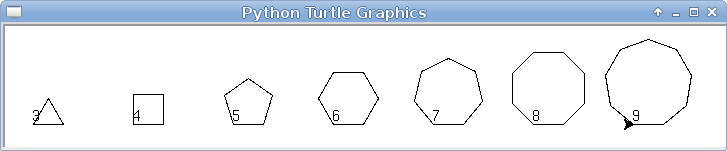
\includegraphics[width=0.8\textwidth]{pave.png}$$

On se déplace donc, crayon levé, jusqu'à l'origine en bas à gauche d'un hexagone,
puis on trace l'hexagone ($c = 6$).
\begin{Verbatim}	
# dessin d'un hexagone
up()
goto(x,y)
down()
for k in range(c) :
    forward(d)
    left(360/c)
\end{Verbatim}

\end{enumerate}

\noindent
\begin{minipage}[t]{7cm}
\paragraph{Résultat} En \python, l'algorithme correspondant, présenté ci-contre, 
est donc composé de 3 boucles imbriquées. 
Il faut inclure le module \texttt{math} pour utiliser la fonction \texttt{sqrt()}
ainsi que le module \texttt{turtle} pour les fonctions de manipulation de la tortue \logo{}
(\texttt{up()}, \texttt{down()}, \texttt{goto()}, \texttt{left()} et \texttt{forward()}).
Pour le tester, on fixera les valeurs de $c$ (nombre de côtés, 6 pour un hexagone),
$d$ (longueur du côté de l'hexagone), $n$ (nombre d'hexagones dans une ligne) et $m$ 
(nombre de lignes) ainsi que l'origine du motif  $(x_0,y_0)$.
Pour le vérifier, on comparera le tracé obtenu avec celui de la figure du motif
présentée plus haut en début de section.
\end{minipage}
\hfill
\begin{minipage}[t]{8.25cm}\footnotesize
\begin{lstlisting}
from math import *
from turtle import *
# initialisation du motif
c, d = 6, 20
n, m = 5, 4
x0, y0 = 0, 0
# dessin du motif
for j in range(m) :
    x, y = x0, y0 + j*d*sqrt(3)
    # dessin d'une ligne d'hexagones
    for i in range(n) :
        x = x0 + 2*i*d
        # dessin d'un hexagone
        up()
        goto(x,y)
        down()
        for k in range(c) :
            forward(d)
            left(360/c)
\end{lstlisting}
\end{minipage}

\paragraph{Vérifications} 
on compare le tracé obtenu lors de l'exécution de l'algorithme précédent avec la figure donnée
en début de section.
\vspace*{3mm}

\noindent\begin{minipage}{6.75cm}
\centerline{\fbox{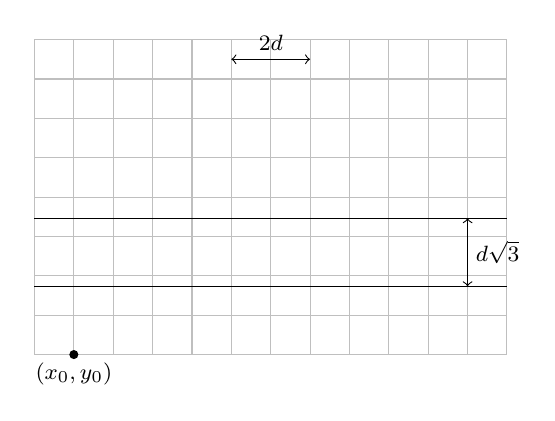
\begin{tikzpicture}[scale=0.5]\footnotesize
\draw[color=lightgray](-6,-4) grid[xstep=1,ystep=1] (6,4);
%\foreach \x in {-6,-5,...,6} \draw(\x,-4) node[below]{\x};
%\foreach \y in {-4,-3,...,4} \draw(-6,\y) node[left]{\y};
%\filldraw(0,0) circle (0.1);
%\draw[->] (-6,0) -- (6,0);
%\draw (6,0) node[right]{$x$} ;
%\draw[->] (0,-4) -- (0,4);
%\draw (0,4) node[above]{$y$};
\foreach \y in {-4,-2.27,-0.53,1.20} \foreach \x in {-5,-3,-1,1,3} \hexagone{\x}{\y} ;
\draw(5,{-4+3*sqrt(3)/2}) node[right]{$d\sqrt{3}$};
\draw (-6,{-4+sqrt(3)}) -- (6,{-4+sqrt(3)});
\draw (-6,{-4+2*sqrt(3)}) -- (6,{-4+2*sqrt(3)});
\draw[<->] (5,{-4+2*sqrt(3)}) -- (5,{-4+sqrt(3)});
\draw(0,3.5) node[above]{$2d$};
\draw[<->] (-1,3.5) -- (1,3.5);
\filldraw(-5,-4) circle (0.1);
\draw(-5,-4) node[below]{$(x_0,y_0)$};
\end{tikzpicture}}}
\centerline{figure de l'énoncé}
\end{minipage}
\hfill
\begin{minipage}{6.25cm}
\centerline{\fbox{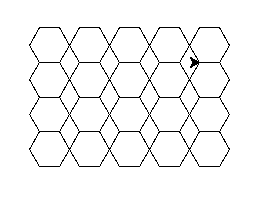
\includegraphics[width=6cm]{pavage.png}}}
\centerline{tracé \python}
\end{minipage}
\vspace*{3mm}

\noindent Les figures sont bien similaires.
%-------------------------------------------------------------------------
\subsubsection{Questions}
%-------------------------------------------------------------------------
En utilisant les instructions de la tortue \logo{}
(module \texttt{turtle}), écrire un algorithme qui dessine un motif géométrique
composé de $(n\times m)$ pavés élémentaires disposés régulièrement sur une grille
ou disposés en quinconce sur la grille.
\vspace*{3mm}

\centerline{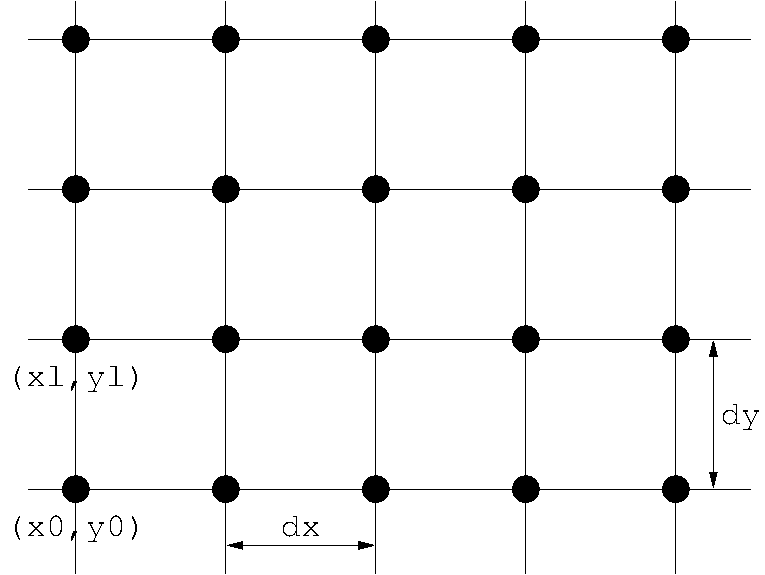
\includegraphics[width=4cm]{grille-1.pdf}\hspace*{1cm}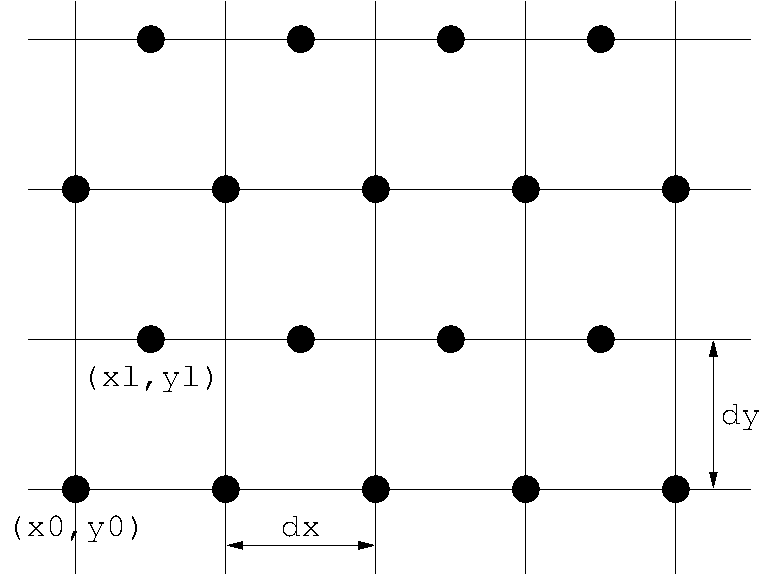
\includegraphics[width=4cm]{grille-2.pdf}}
\centerline{\makebox[4cm]{alignés}\hspace*{1cm}\makebox[4cm]{en quinconce}}

\begin{minipage}[t]{7cm}
\begin{enumerate}
\item \begin{minipage}{1.75cm}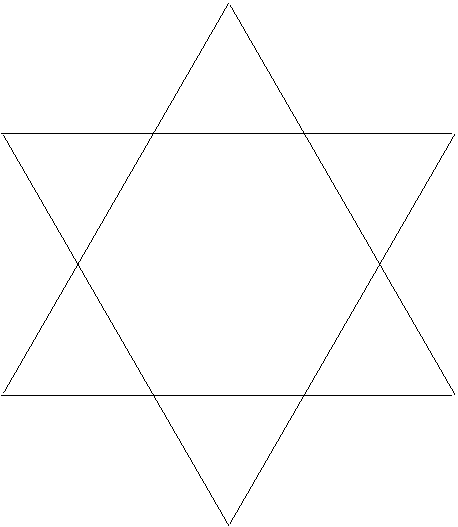
\includegraphics[height=1cm]{etoile-1.pdf}\end{minipage} alignés
\item \begin{minipage}{1.75cm}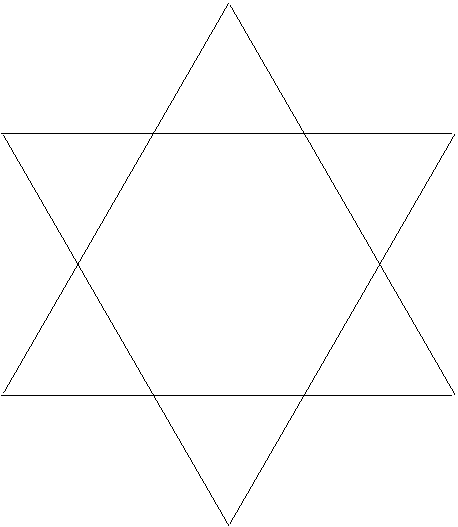
\includegraphics[height=1cm]{etoile-1.pdf}\end{minipage} en quinconce
\item \begin{minipage}{1.75cm}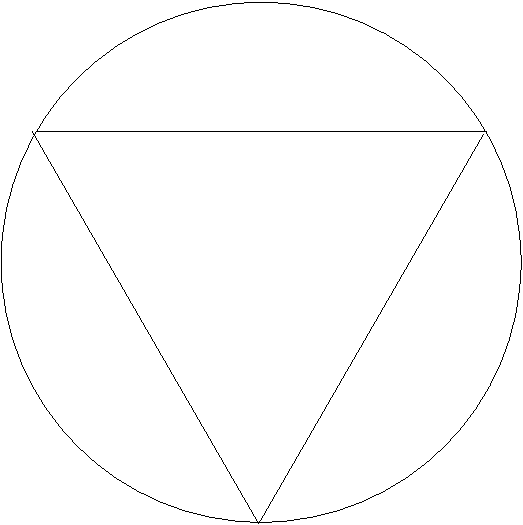
\includegraphics[height=1cm]{cercle-1.pdf}\end{minipage} alignés
\item \begin{minipage}{1.75cm}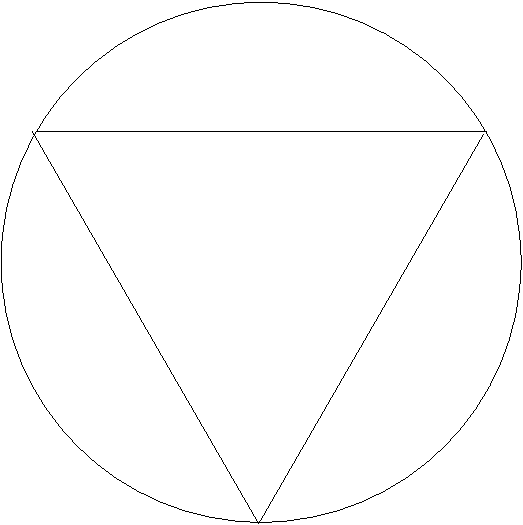
\includegraphics[height=1cm]{cercle-1.pdf}\end{minipage} en quinconce
\item \begin{minipage}{1.75cm}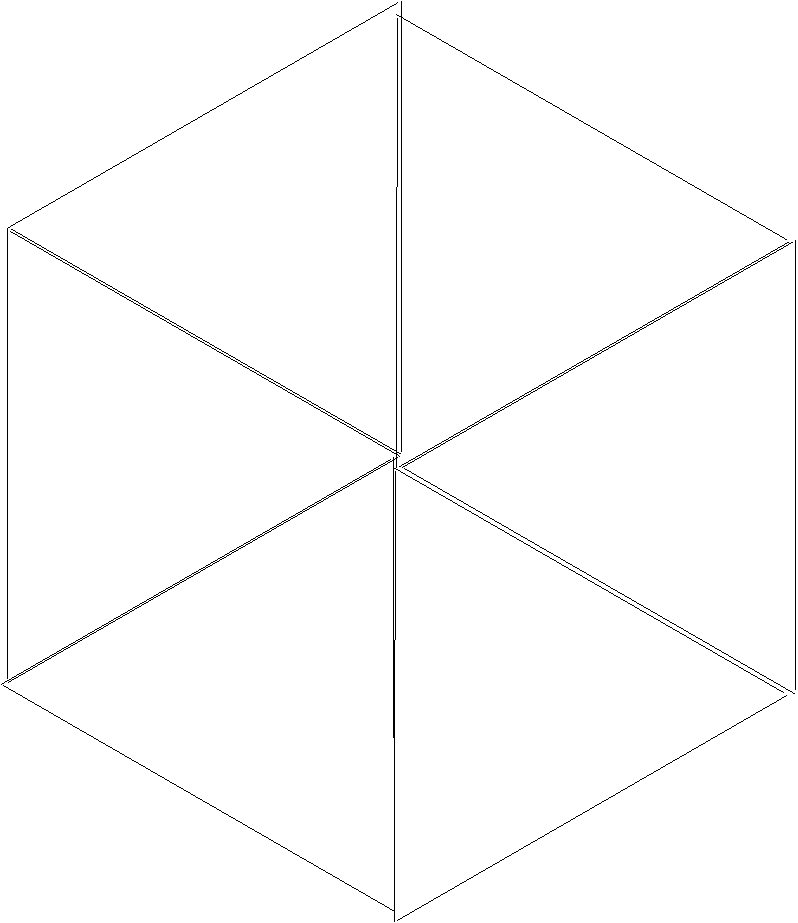
\includegraphics[height=1cm]{hexagone-1.pdf}\end{minipage} alignés
\item \begin{minipage}{1.75cm}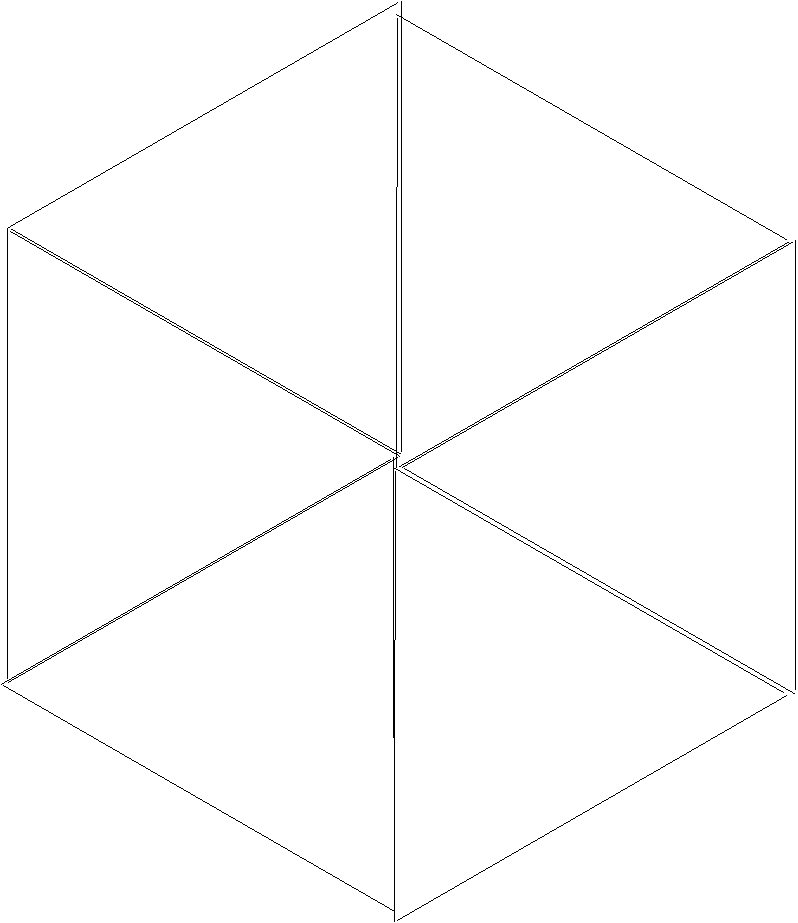
\includegraphics[height=1cm]{hexagone-1.pdf}\end{minipage} en quinconce
\item \begin{minipage}{1.75cm}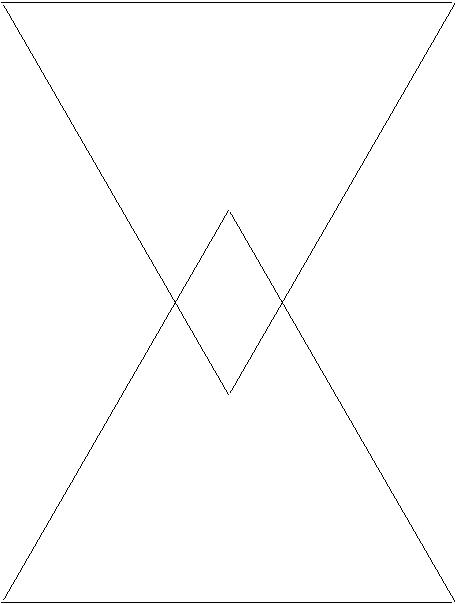
\includegraphics[height=1cm]{triangle-1.pdf}\end{minipage} alignés
\item \begin{minipage}{1.75cm}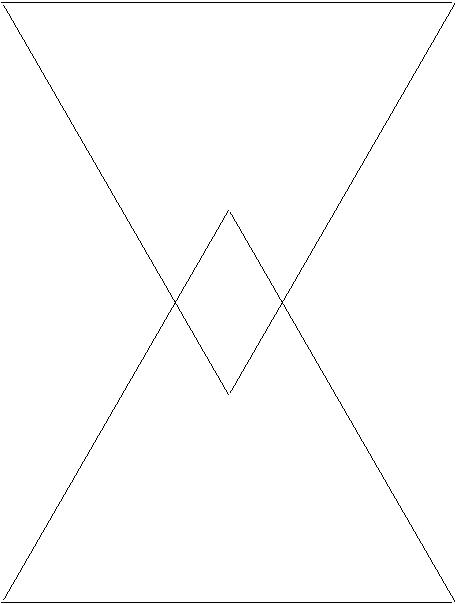
\includegraphics[height=1cm]{triangle-1.pdf}\end{minipage} en quinconce
\item \begin{minipage}{1.75cm}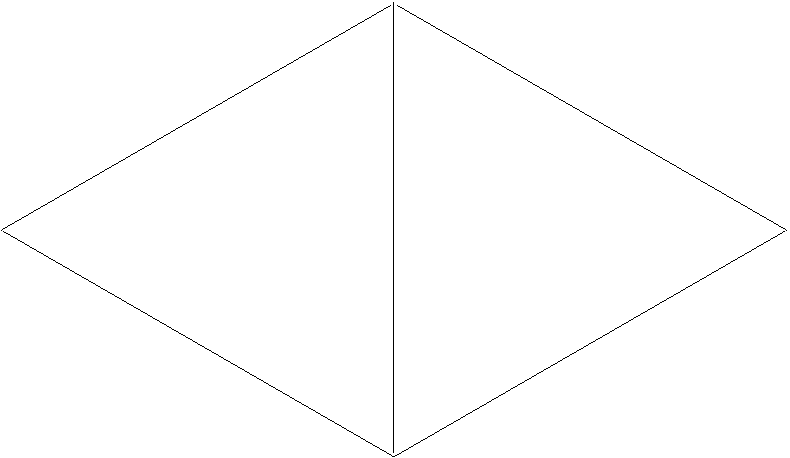
\includegraphics[height=1cm]{losange-1.pdf}\end{minipage} alignés
\item \begin{minipage}{1.75cm}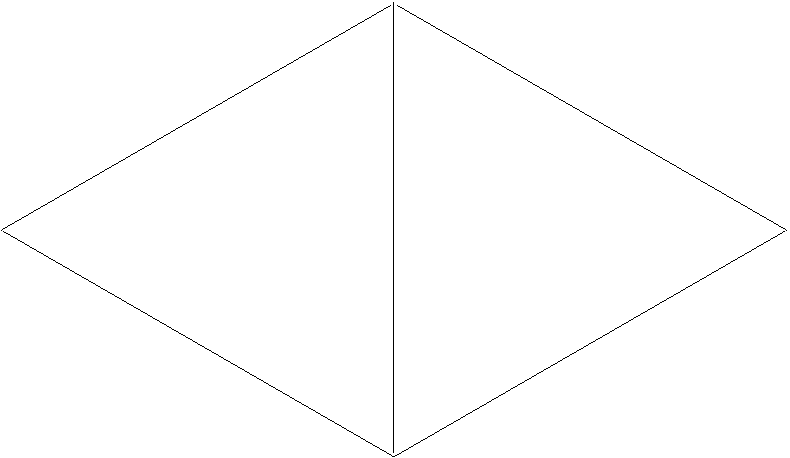
\includegraphics[height=1cm]{losange-1.pdf}\end{minipage} en quinconce
\item \begin{minipage}{1.75cm}
\includegraphics[height=1cm]{carre-1.pdf}\end{minipage} alignés
\item \begin{minipage}{1.75cm}
\includegraphics[height=1cm]{carre-1.pdf}\end{minipage} en quinconce
\end{enumerate}
\end{minipage}
\hfill
\begin{minipage}[t]{7cm}
\begin{enumerate}\setcounter{enumi}{12}
\item \begin{minipage}{1.75cm}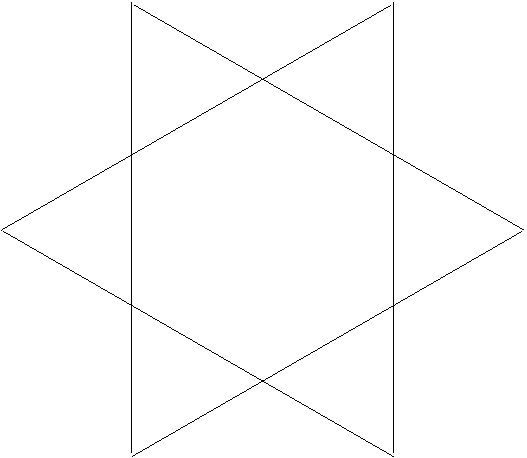
\includegraphics[height=1cm]{etoile-2.pdf}\end{minipage} alignés
\item \begin{minipage}{1.75cm}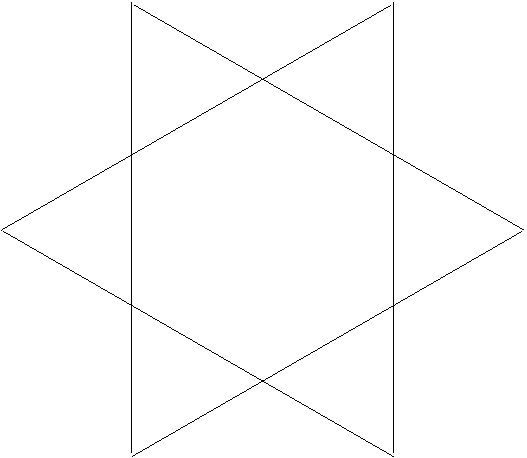
\includegraphics[height=1cm]{etoile-2.pdf}\end{minipage} en quinconce
\item \begin{minipage}{1.75cm}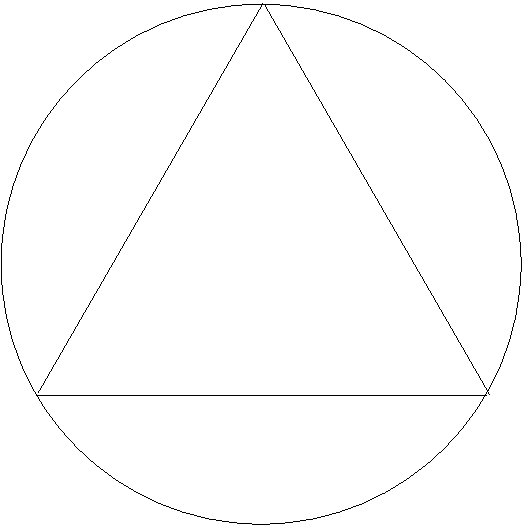
\includegraphics[height=1cm]{cercle-2.pdf}\end{minipage} alignés
\item \begin{minipage}{1.75cm}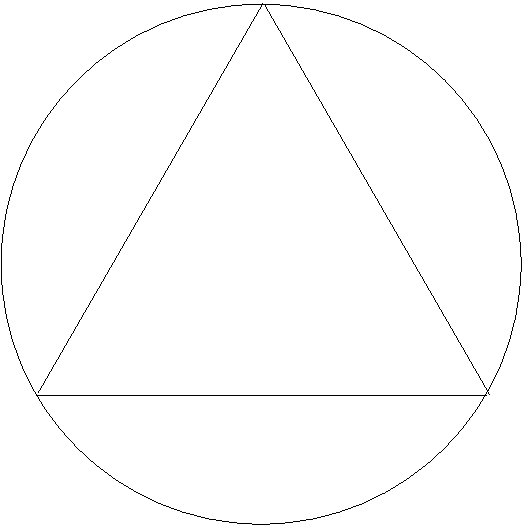
\includegraphics[height=1cm]{cercle-2.pdf}\end{minipage} en quinconce
\item \begin{minipage}{1.75cm}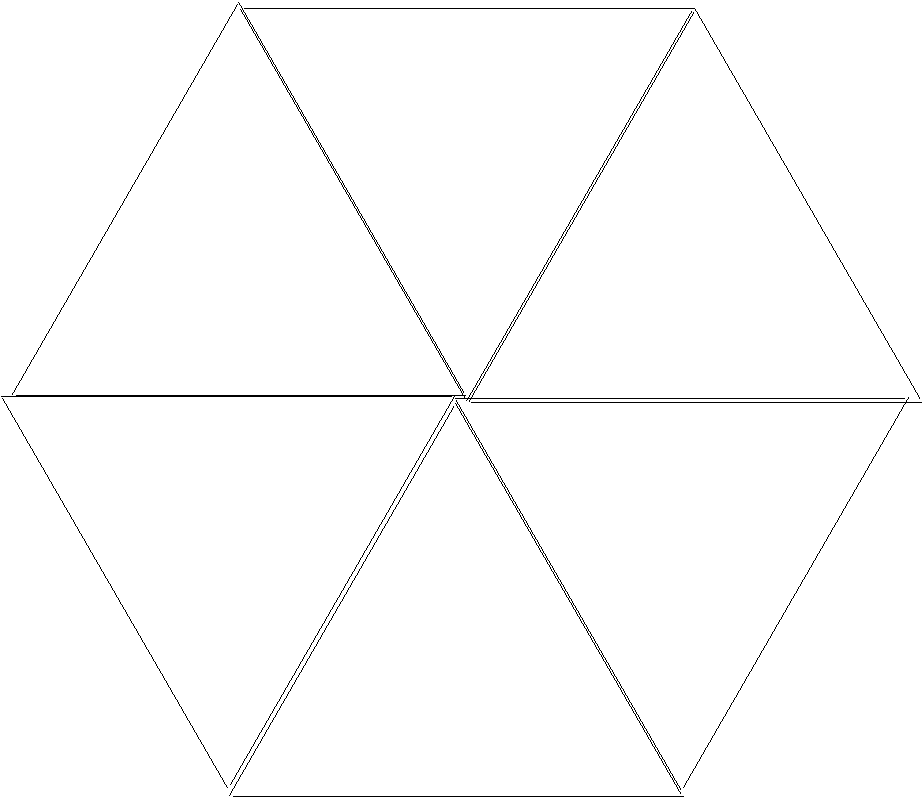
\includegraphics[height=1cm]{hexagone-2.pdf}\end{minipage} alignés
\item \begin{minipage}{1.75cm}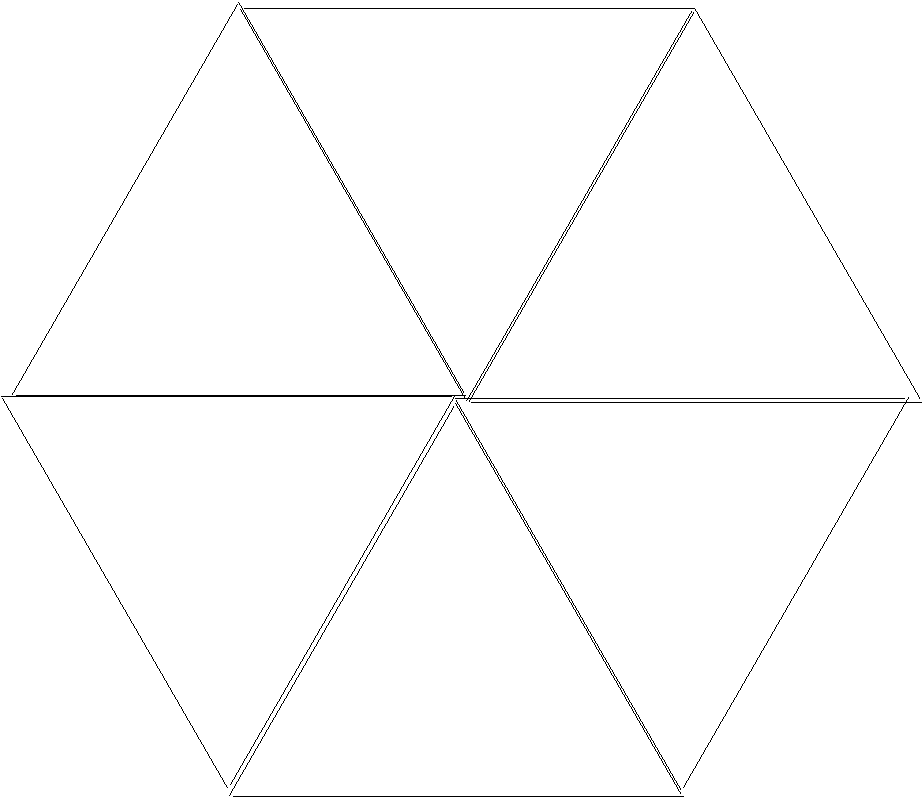
\includegraphics[height=1cm]{hexagone-2.pdf}\end{minipage} en quinconce
\item \begin{minipage}{1.75cm}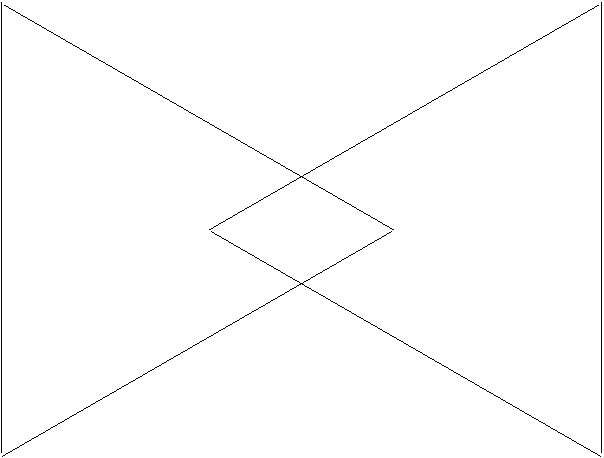
\includegraphics[height=1cm]{triangle-2.pdf}\end{minipage} alignés
\item \begin{minipage}{1.75cm}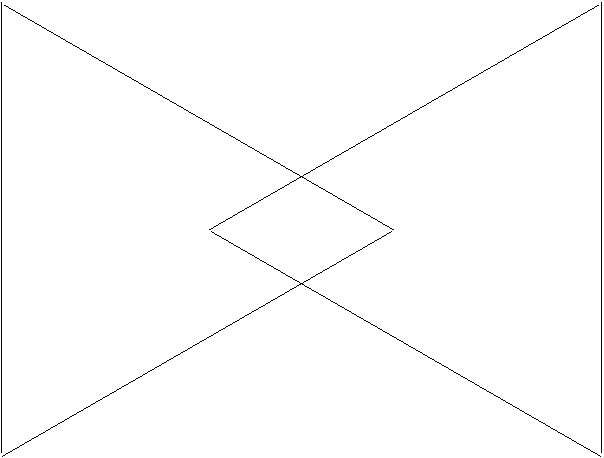
\includegraphics[height=1cm]{triangle-2.pdf}\end{minipage} en quinconce
\item \begin{minipage}{1.75cm}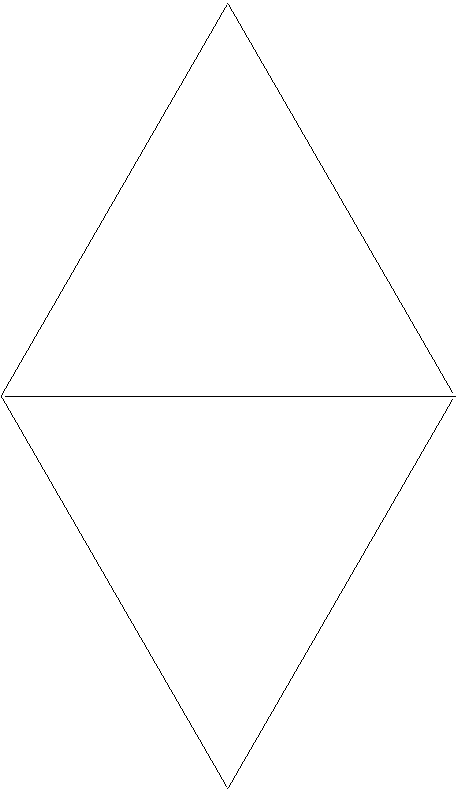
\includegraphics[height=1cm]{losange-2.pdf}\end{minipage} alignés
\item \begin{minipage}{1.75cm}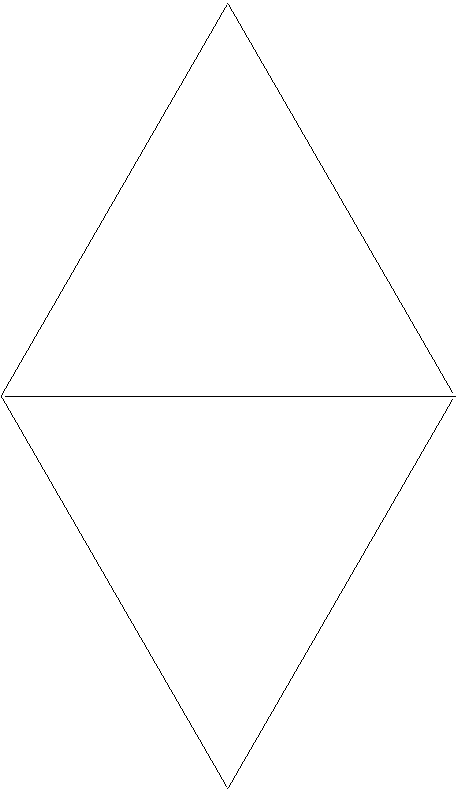
\includegraphics[height=1cm]{losange-2.pdf}\end{minipage} en quinconce
\item \begin{minipage}{1.75cm}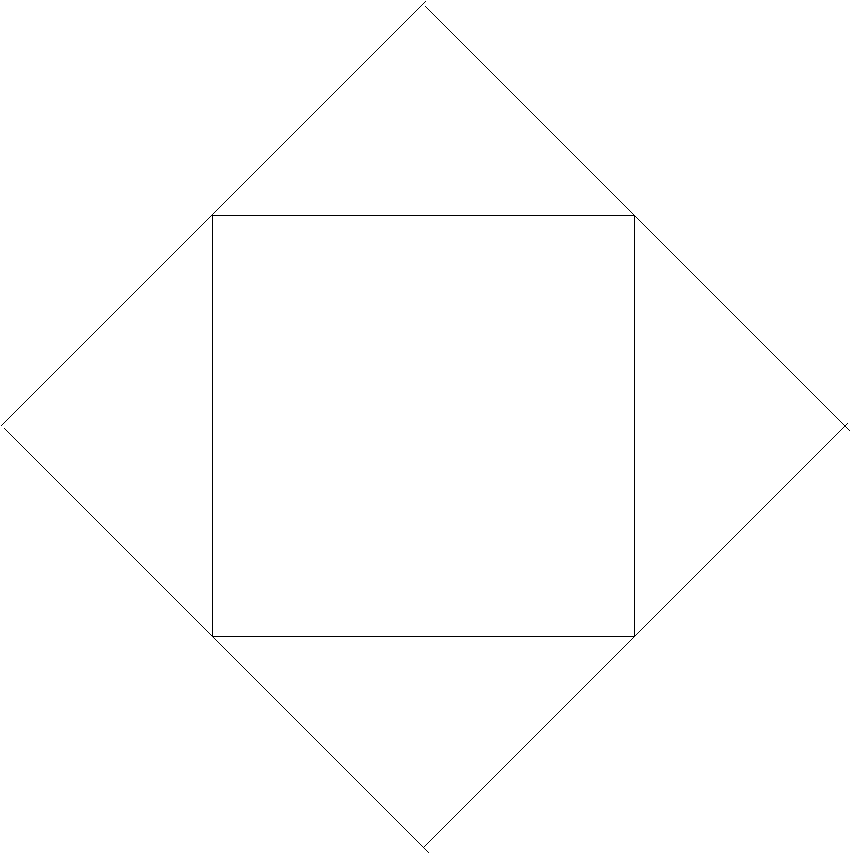
\includegraphics[height=1cm]{carre-2.pdf}\end{minipage} alignés
\item \begin{minipage}{1.75cm}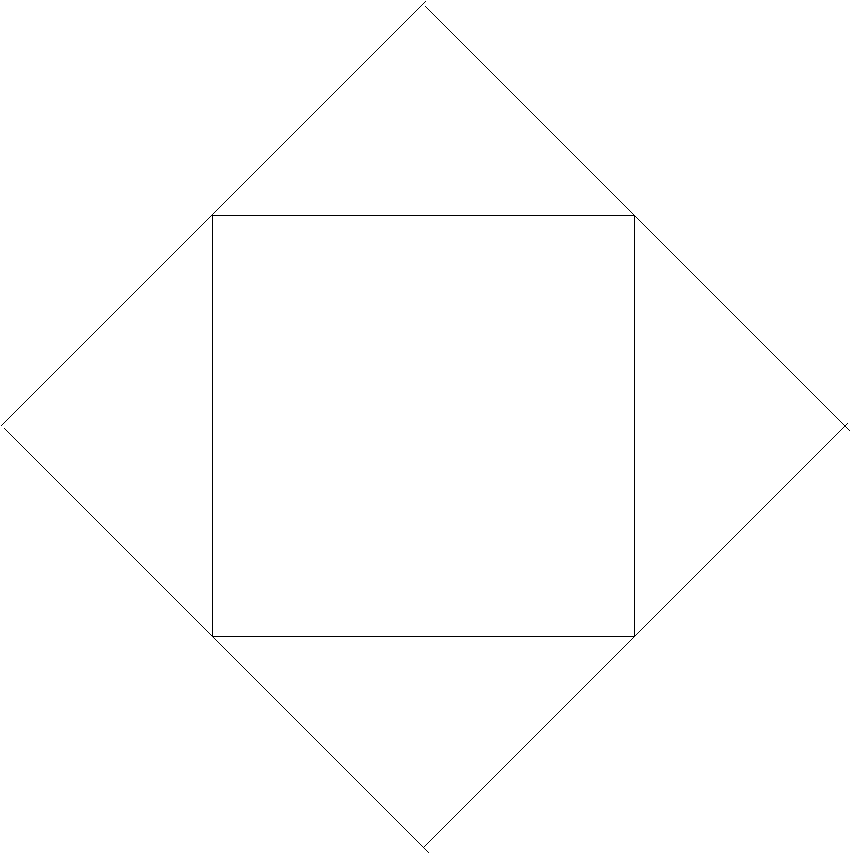
\includegraphics[height=1cm]{carre-2.pdf}\end{minipage} en quinconce
\end{enumerate}
\end{minipage}

%-------------------------------------------------------------------------
\subsection{Révisions}
%-------------------------------------------------------------------------

$$\begin{tabular}{|ll@{ : }l|}
\hline
\textbf{Cours} & \cite{cours} & chapitre 2, sections 2.4.2 à 2.4.4 \\
\textbf{TD}    & \cite{td}    & exercices 2.20 à 2.24 et 2.34 \\
\hline
\end{tabular}$$
